\begin{frame}
    \frametitle{FHR Benchmark Specifications}
    \begin{itemize}
        \item UIUC participates in the benchmark with OpenMC
    \end{itemize}
    \vspace{-0.2cm}
    \begin{table}
        \caption{OECD NEA's FHR Benchmark Phases 
        \cite{petrovic_benchmark_2021}.}
        \vspace{-0.25cm}
        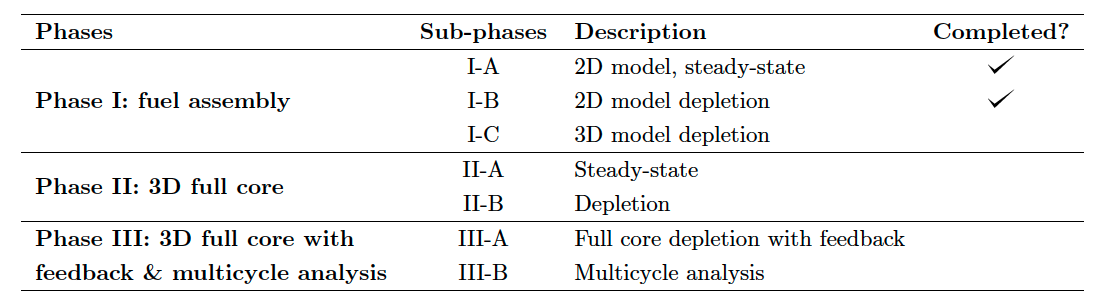
\includegraphics[width=0.9\linewidth]{figures/benchmark-phases.png} 
    \end{table}
    \vspace{-0.3cm}
    \begin{figure}[]
        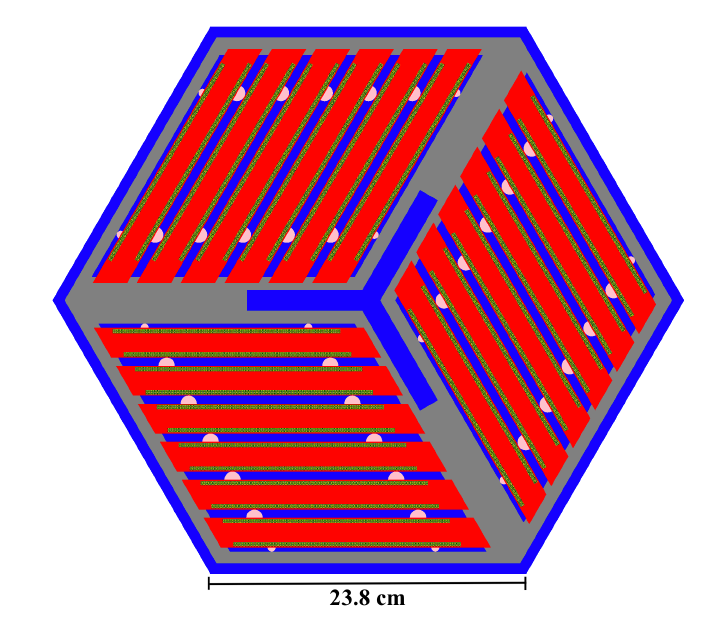
\includegraphics[width=0.3\linewidth]{figures/ahtr-assembly.png} 
        \caption{AHTR fuel assembly.}
    \end{figure}
\end{frame}

\begin{frame}
    \frametitle{FHR Benchmark Specifications}
    \begin{itemize}
        \item Only Phase I-A and I-B specifications have been released 
        \item Benchmark participants must produce the following results for 
        the 9 cases: $k_{eff}$, reactivity coefficients ($\beta_{eff}$, 
        $\alpha_D$, $\alpha_{T, FliBe}$, $\alpha_M$), fission source distribution, 
        neutron flux distribution, fuel assembly averaged neutron spectrum
    \end{itemize}
    \vspace{-0.25cm}
    \begin{table}
        \caption{Description of the \acrlong{FHR} benchmark Phase I-A cases 
        \vspace{-0.25cm}
        \cite{noauthor_fluoride_nodate}.}
        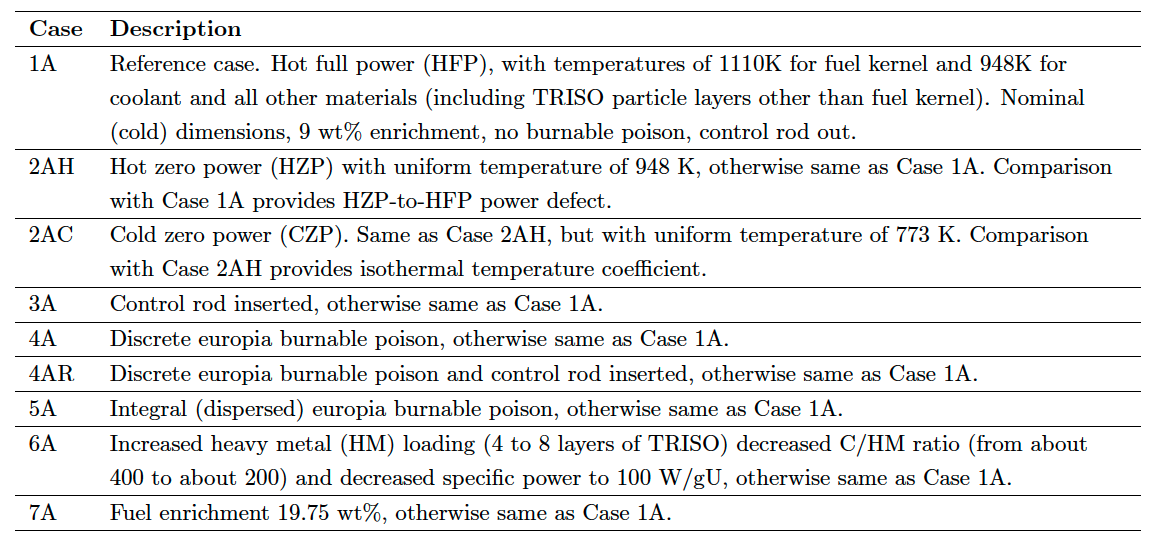
\includegraphics[width=0.6\linewidth]{figures/benchmark-cases.png} 
    \end{table}
\end{frame}